\documentclass[12pt]{article}
\usepackage{tikz}
\usepackage{amsmath}
% Underlining package
\usepackage{ulem}
\usetikzlibrary{calc}
\usepackage[a4paper, portrait, margin=1cm]{geometry}
\usepackage{fancyhdr}

\def \HeadingQuestions {\section*{\Large Name: \underline{\hspace{8cm}} \hfill Date: \underline{\hspace{3cm}}} \vspace{-3mm}
{Angles in a Triangle: Questions} \vspace{1pt}\hrule}

% raise footer with page number; no header
\fancypagestyle{myfancypagestyle}{
  \fancyhf{}% clear all header and footer fields
  \renewcommand{\headrulewidth}{0pt} % no rule under header
  \fancyfoot[C] {\thepage} \setlength{\footskip}{14.5pt} % raise page number 6pt
}
\pagestyle{myfancypagestyle}  % apply myfancypagestyle

\newcounter{minipagecount}

\begin{document}
\HeadingQuestions
\vspace{8mm}

\begin{minipage}{0.55\textwidth}
  \refstepcounter{minipagecount}
  \noindent{(\theminipagecount)}\quad
  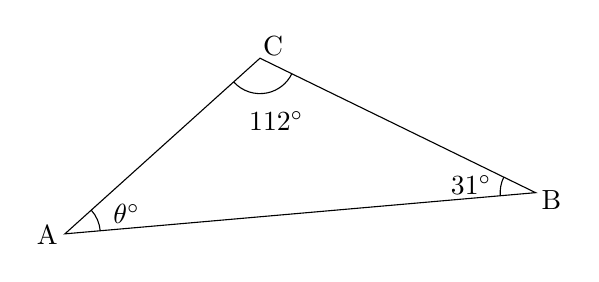
\begin{tikzpicture}[scale=1.5, baseline=(current bounding box.north)]
      \pgfmathsetmacro{\angleA}{37}
      \pgfmathsetmacro{\angleB}{31}
      \pgfmathsetmacro{\angleC}{112}
      \pgfmathsetmacro{\sideC}{4}
      \pgfmathsetmacro{\rotationAngle}{5}


      \begin{scope}[rotate=\rotationAngle]
        \coordinate (A) at (0,0);
        \coordinate (B) at (\sideC,0);
        \coordinate (C) at (intersection cs: first line={(A)--($(A)+(\angleA:4cm)$)}, second line={(B)--($(B)+(180-\angleB:4cm)$)});
        \draw (A) -- (B) -- (C) -- cycle;

        % Mark angles with arcs
        \draw ($(A)!0.3cm!(B)$) arc [start angle=0, end angle=\angleA, radius=0.3cm];
        \draw ($(B)!0.3cm!(C)$) arc [start angle=180-\angleB, end angle=180, radius=0.3cm];
        \draw ($(C)!0.3cm!(A)$) arc [start angle=180+\angleA, end angle=360-\angleB, radius=0.3cm];

        % Label angles
        \node at ($(A)!-0.15cm!(B)$) {A};
        \node at ($(B)!-0.15cm!(C)$) {B};
        \node at ($(C)!-0.15cm!(A)$) {C};

        % Mark angles in degrees
        \coordinate (midBC) at ($(B)!0.5!(C)$);
        \node at ($(A)!0.55cm!(midBC)$) {$\theta ^\circ$};

        \coordinate (midAC) at ($(A)!0.5!(C)$);
        \node at ($(B)!0.55cm!(midAC)$) {31$^\circ$};

        \coordinate (midAB) at ($(A)!0.5!(B)$);
        \node at ($(C)!0.55cm!(midAB)$) {112$^\circ$};

      \end{scope}
    \end{tikzpicture}
\end{minipage}%
\hfill
\begin{minipage}{0.4\textwidth}
    \begin{align*}
        \angle \text{A} &= 180^\circ - (\angle \text{B} + \angle \text{C}) \\
        &= 180^\circ - (\dotuline{~~~~~~~}^\circ + \dotuline{~~~~~~~}^\circ) \\
        &= 180^\circ - \dotuline{~~~~~~~}^\circ \\
        &= \dotuline{~~~~~~~}^\circ
    \end{align*}
\end{minipage}

\vspace{1cm}\begin{minipage}{0.55\textwidth}
  \refstepcounter{minipagecount}
  \noindent{(\theminipagecount)}\quad
  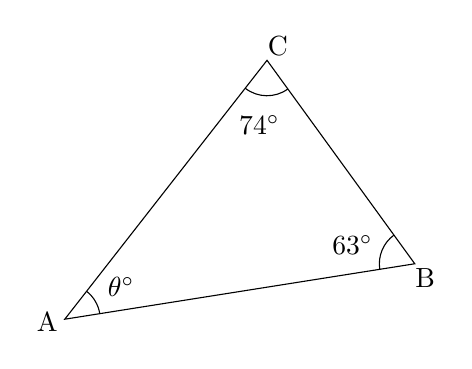
\begin{tikzpicture}[scale=1.5, baseline=(current bounding box.north)]
      \pgfmathsetmacro{\angleA}{43}
      \pgfmathsetmacro{\angleB}{63}
      \pgfmathsetmacro{\angleC}{74}
      \pgfmathsetmacro{\sideC}{3}
      \pgfmathsetmacro{\rotationAngle}{9}


      \begin{scope}[rotate=\rotationAngle]
        \coordinate (A) at (0,0);
        \coordinate (B) at (\sideC,0);
        \coordinate (C) at (intersection cs: first line={(A)--($(A)+(\angleA:4cm)$)}, second line={(B)--($(B)+(180-\angleB:4cm)$)});
        \draw (A) -- (B) -- (C) -- cycle;

        % Mark angles with arcs
        \draw ($(A)!0.3cm!(B)$) arc [start angle=0, end angle=\angleA, radius=0.3cm];
        \draw ($(B)!0.3cm!(C)$) arc [start angle=180-\angleB, end angle=180, radius=0.3cm];
        \draw ($(C)!0.3cm!(A)$) arc [start angle=180+\angleA, end angle=360-\angleB, radius=0.3cm];

        % Label angles
        \node at ($(A)!-0.15cm!(B)$) {A};
        \node at ($(B)!-0.15cm!(C)$) {B};
        \node at ($(C)!-0.15cm!(A)$) {C};

        % Mark angles in degrees
        \coordinate (midBC) at ($(B)!0.5!(C)$);
        \node at ($(A)!0.55cm!(midBC)$) {$\theta ^\circ$};

        \coordinate (midAC) at ($(A)!0.5!(C)$);
        \node at ($(B)!0.55cm!(midAC)$) {63$^\circ$};

        \coordinate (midAB) at ($(A)!0.5!(B)$);
        \node at ($(C)!0.55cm!(midAB)$) {74$^\circ$};

      \end{scope}
    \end{tikzpicture}
\end{minipage}%
\hfill
\begin{minipage}{0.4\textwidth}
    \begin{align*}
        \angle \text{A} &= 180^\circ - (\angle \text{B} + \angle \text{C}) \\
        &= 180^\circ - (\dotuline{~~~~~~~}^\circ + \dotuline{~~~~~~~}^\circ) \\
        &= 180^\circ - \dotuline{~~~~~~~}^\circ \\
        &= \dotuline{~~~~~~~}^\circ
    \end{align*}
\end{minipage}

\vspace{1cm}\begin{minipage}{0.55\textwidth}
  \refstepcounter{minipagecount}
  \noindent{(\theminipagecount)}\quad
  \begin{tikzpicture}[scale=1.5, baseline=(current bounding box.north)]
      \pgfmathsetmacro{\angleA}{56}
      \pgfmathsetmacro{\angleB}{44}
      \pgfmathsetmacro{\angleC}{80}
      \pgfmathsetmacro{\sideC}{4}
      \pgfmathsetmacro{\rotationAngle}{7}


      \begin{scope}[rotate=\rotationAngle]
        \coordinate (A) at (0,0);
        \coordinate (B) at (\sideC,0);
        \coordinate (C) at (intersection cs: first line={(A)--($(A)+(\angleA:4cm)$)}, second line={(B)--($(B)+(180-\angleB:4cm)$)});
        \draw (A) -- (B) -- (C) -- cycle;

        % Mark angles with arcs
        \draw ($(A)!0.3cm!(B)$) arc [start angle=0, end angle=\angleA, radius=0.3cm];
        \draw ($(B)!0.3cm!(C)$) arc [start angle=180-\angleB, end angle=180, radius=0.3cm];
        \draw ($(C)!0.3cm!(A)$) arc [start angle=180+\angleA, end angle=360-\angleB, radius=0.3cm];

        % Label angles
        \node at ($(A)!-0.15cm!(B)$) {A};
        \node at ($(B)!-0.15cm!(C)$) {B};
        \node at ($(C)!-0.15cm!(A)$) {C};

        % Mark angles in degrees
        \coordinate (midBC) at ($(B)!0.5!(C)$);
        \node at ($(A)!0.55cm!(midBC)$) {$\theta ^\circ$};

        \coordinate (midAC) at ($(A)!0.5!(C)$);
        \node at ($(B)!0.55cm!(midAC)$) {44$^\circ$};

        \coordinate (midAB) at ($(A)!0.5!(B)$);
        \node at ($(C)!0.55cm!(midAB)$) {80$^\circ$};

      \end{scope}
    \end{tikzpicture}
\end{minipage}%
\hfill
\begin{minipage}{0.4\textwidth}
    \begin{align*}
        \angle \text{A} &= 180^\circ - (\angle \text{B} + \angle \text{C}) \\
        &= 180^\circ - (\dotuline{~~~~~~~}^\circ + \dotuline{~~~~~~~}^\circ) \\
        &= 180^\circ - \dotuline{~~~~~~~}^\circ \\
        &= \dotuline{~~~~~~~}^\circ
    \end{align*}
\end{minipage}

\vspace{1cm}\begin{minipage}{0.55\textwidth}
  \refstepcounter{minipagecount}
  \noindent{(\theminipagecount)}\quad
  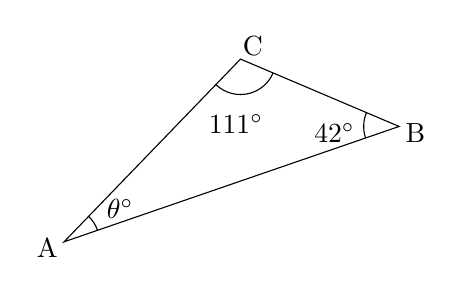
\begin{tikzpicture}[scale=1.5, baseline=(current bounding box.north)]
      \pgfmathsetmacro{\angleA}{27}
      \pgfmathsetmacro{\angleB}{42}
      \pgfmathsetmacro{\angleC}{111}
      \pgfmathsetmacro{\sideC}{3}
      \pgfmathsetmacro{\rotationAngle}{19}


      \begin{scope}[rotate=\rotationAngle]
        \coordinate (A) at (0,0);
        \coordinate (B) at (\sideC,0);
        \coordinate (C) at (intersection cs: first line={(A)--($(A)+(\angleA:4cm)$)}, second line={(B)--($(B)+(180-\angleB:4cm)$)});
        \draw (A) -- (B) -- (C) -- cycle;

        % Mark angles with arcs
        \draw ($(A)!0.3cm!(B)$) arc [start angle=0, end angle=\angleA, radius=0.3cm];
        \draw ($(B)!0.3cm!(C)$) arc [start angle=180-\angleB, end angle=180, radius=0.3cm];
        \draw ($(C)!0.3cm!(A)$) arc [start angle=180+\angleA, end angle=360-\angleB, radius=0.3cm];

        % Label angles
        \node at ($(A)!-0.15cm!(B)$) {A};
        \node at ($(B)!-0.15cm!(C)$) {B};
        \node at ($(C)!-0.15cm!(A)$) {C};

        % Mark angles in degrees
        \coordinate (midBC) at ($(B)!0.5!(C)$);
        \node at ($(A)!0.55cm!(midBC)$) {$\theta ^\circ$};

        \coordinate (midAC) at ($(A)!0.5!(C)$);
        \node at ($(B)!0.55cm!(midAC)$) {42$^\circ$};

        \coordinate (midAB) at ($(A)!0.5!(B)$);
        \node at ($(C)!0.55cm!(midAB)$) {111$^\circ$};

      \end{scope}
    \end{tikzpicture}
\end{minipage}%
\hfill
\begin{minipage}{0.4\textwidth}
    \begin{align*}
        \angle \text{A} &= 180^\circ - (\angle \text{B} + \angle \text{C}) \\
        &= 180^\circ - (\dotuline{~~~~~~~}^\circ + \dotuline{~~~~~~~}^\circ) \\
        &= 180^\circ - \dotuline{~~~~~~~}^\circ \\
        &= \dotuline{~~~~~~~}^\circ
    \end{align*}
\end{minipage}

\vspace{1cm}\begin{minipage}{0.55\textwidth}
  \refstepcounter{minipagecount}
  \noindent{(\theminipagecount)}\quad
  \begin{tikzpicture}[scale=1.5, baseline=(current bounding box.north)]
      \pgfmathsetmacro{\angleA}{29}
      \pgfmathsetmacro{\angleB}{54}
      \pgfmathsetmacro{\angleC}{97}
      \pgfmathsetmacro{\sideC}{4}
      \pgfmathsetmacro{\rotationAngle}{20}


      \begin{scope}[rotate=\rotationAngle]
        \coordinate (A) at (0,0);
        \coordinate (B) at (\sideC,0);
        \coordinate (C) at (intersection cs: first line={(A)--($(A)+(\angleA:4cm)$)}, second line={(B)--($(B)+(180-\angleB:4cm)$)});
        \draw (A) -- (B) -- (C) -- cycle;

        % Mark angles with arcs
        \draw ($(A)!0.3cm!(B)$) arc [start angle=0, end angle=\angleA, radius=0.3cm];
        \draw ($(B)!0.3cm!(C)$) arc [start angle=180-\angleB, end angle=180, radius=0.3cm];
        \draw ($(C)!0.3cm!(A)$) arc [start angle=180+\angleA, end angle=360-\angleB, radius=0.3cm];

        % Label angles
        \node at ($(A)!-0.15cm!(B)$) {A};
        \node at ($(B)!-0.15cm!(C)$) {B};
        \node at ($(C)!-0.15cm!(A)$) {C};

        % Mark angles in degrees
        \coordinate (midBC) at ($(B)!0.5!(C)$);
        \node at ($(A)!0.55cm!(midBC)$) {$\theta ^\circ$};

        \coordinate (midAC) at ($(A)!0.5!(C)$);
        \node at ($(B)!0.55cm!(midAC)$) {54$^\circ$};

        \coordinate (midAB) at ($(A)!0.5!(B)$);
        \node at ($(C)!0.55cm!(midAB)$) {97$^\circ$};

      \end{scope}
    \end{tikzpicture}
\end{minipage}%
\hfill
\begin{minipage}{0.4\textwidth}
    \begin{align*}
        \angle \text{A} &= 180^\circ - (\angle \text{B} + \angle \text{C}) \\
        &= 180^\circ - (\dotuline{~~~~~~~}^\circ + \dotuline{~~~~~~~}^\circ) \\
        &= 180^\circ - \dotuline{~~~~~~~}^\circ \\
        &= \dotuline{~~~~~~~}^\circ
    \end{align*}
\end{minipage}

\vspace{1cm}\begin{minipage}{0.55\textwidth}
  \refstepcounter{minipagecount}
  \noindent{(\theminipagecount)}\quad
  \begin{tikzpicture}[scale=1.5, baseline=(current bounding box.north)]
      \pgfmathsetmacro{\angleA}{44}
      \pgfmathsetmacro{\angleB}{35}
      \pgfmathsetmacro{\angleC}{101}
      \pgfmathsetmacro{\sideC}{4}
      \pgfmathsetmacro{\rotationAngle}{19}


      \begin{scope}[rotate=\rotationAngle]
        \coordinate (A) at (0,0);
        \coordinate (B) at (\sideC,0);
        \coordinate (C) at (intersection cs: first line={(A)--($(A)+(\angleA:4cm)$)}, second line={(B)--($(B)+(180-\angleB:4cm)$)});
        \draw (A) -- (B) -- (C) -- cycle;

        % Mark angles with arcs
        \draw ($(A)!0.3cm!(B)$) arc [start angle=0, end angle=\angleA, radius=0.3cm];
        \draw ($(B)!0.3cm!(C)$) arc [start angle=180-\angleB, end angle=180, radius=0.3cm];
        \draw ($(C)!0.3cm!(A)$) arc [start angle=180+\angleA, end angle=360-\angleB, radius=0.3cm];

        % Label angles
        \node at ($(A)!-0.15cm!(B)$) {A};
        \node at ($(B)!-0.15cm!(C)$) {B};
        \node at ($(C)!-0.15cm!(A)$) {C};

        % Mark angles in degrees
        \coordinate (midBC) at ($(B)!0.5!(C)$);
        \node at ($(A)!0.55cm!(midBC)$) {$\theta ^\circ$};

        \coordinate (midAC) at ($(A)!0.5!(C)$);
        \node at ($(B)!0.55cm!(midAC)$) {35$^\circ$};

        \coordinate (midAB) at ($(A)!0.5!(B)$);
        \node at ($(C)!0.55cm!(midAB)$) {101$^\circ$};

      \end{scope}
    \end{tikzpicture}
\end{minipage}%
\hfill
\begin{minipage}{0.4\textwidth}
    \begin{align*}
        \angle \text{A} &= 180^\circ - (\angle \text{B} + \angle \text{C}) \\
        &= 180^\circ - (\dotuline{~~~~~~~}^\circ + \dotuline{~~~~~~~}^\circ) \\
        &= 180^\circ - \dotuline{~~~~~~~}^\circ \\
        &= \dotuline{~~~~~~~}^\circ
    \end{align*}
\end{minipage}

\vspace{1cm}\begin{minipage}{0.55\textwidth}
  \refstepcounter{minipagecount}
  \noindent{(\theminipagecount)}\quad
  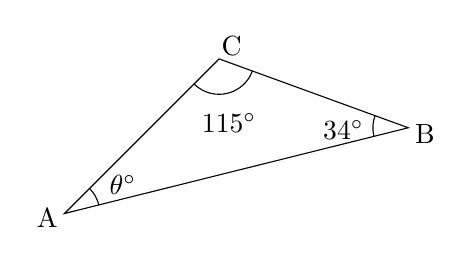
\begin{tikzpicture}[scale=1.5, baseline=(current bounding box.north)]
      \pgfmathsetmacro{\angleA}{31}
      \pgfmathsetmacro{\angleB}{34}
      \pgfmathsetmacro{\angleC}{115}
      \pgfmathsetmacro{\sideC}{3}
      \pgfmathsetmacro{\rotationAngle}{14}


      \begin{scope}[rotate=\rotationAngle]
        \coordinate (A) at (0,0);
        \coordinate (B) at (\sideC,0);
        \coordinate (C) at (intersection cs: first line={(A)--($(A)+(\angleA:4cm)$)}, second line={(B)--($(B)+(180-\angleB:4cm)$)});
        \draw (A) -- (B) -- (C) -- cycle;

        % Mark angles with arcs
        \draw ($(A)!0.3cm!(B)$) arc [start angle=0, end angle=\angleA, radius=0.3cm];
        \draw ($(B)!0.3cm!(C)$) arc [start angle=180-\angleB, end angle=180, radius=0.3cm];
        \draw ($(C)!0.3cm!(A)$) arc [start angle=180+\angleA, end angle=360-\angleB, radius=0.3cm];

        % Label angles
        \node at ($(A)!-0.15cm!(B)$) {A};
        \node at ($(B)!-0.15cm!(C)$) {B};
        \node at ($(C)!-0.15cm!(A)$) {C};

        % Mark angles in degrees
        \coordinate (midBC) at ($(B)!0.5!(C)$);
        \node at ($(A)!0.55cm!(midBC)$) {$\theta ^\circ$};

        \coordinate (midAC) at ($(A)!0.5!(C)$);
        \node at ($(B)!0.55cm!(midAC)$) {34$^\circ$};

        \coordinate (midAB) at ($(A)!0.5!(B)$);
        \node at ($(C)!0.55cm!(midAB)$) {115$^\circ$};

      \end{scope}
    \end{tikzpicture}
\end{minipage}%
\hfill
\begin{minipage}{0.4\textwidth}
    \begin{align*}
        \angle \text{A} &= 180^\circ - (\angle \text{B} + \angle \text{C}) \\
        &= 180^\circ - (\dotuline{~~~~~~~}^\circ + \dotuline{~~~~~~~}^\circ) \\
        &= 180^\circ - \dotuline{~~~~~~~}^\circ \\
        &= \dotuline{~~~~~~~}^\circ
    \end{align*}
\end{minipage}

\vspace{1cm}\begin{minipage}{0.55\textwidth}
  \refstepcounter{minipagecount}
  \noindent{(\theminipagecount)}\quad
  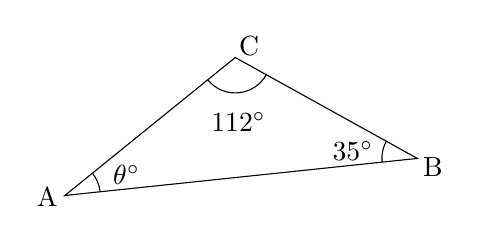
\begin{tikzpicture}[scale=1.5, baseline=(current bounding box.north)]
      \pgfmathsetmacro{\angleA}{33}
      \pgfmathsetmacro{\angleB}{35}
      \pgfmathsetmacro{\angleC}{112}
      \pgfmathsetmacro{\sideC}{3}
      \pgfmathsetmacro{\rotationAngle}{6}


      \begin{scope}[rotate=\rotationAngle]
        \coordinate (A) at (0,0);
        \coordinate (B) at (\sideC,0);
        \coordinate (C) at (intersection cs: first line={(A)--($(A)+(\angleA:4cm)$)}, second line={(B)--($(B)+(180-\angleB:4cm)$)});
        \draw (A) -- (B) -- (C) -- cycle;

        % Mark angles with arcs
        \draw ($(A)!0.3cm!(B)$) arc [start angle=0, end angle=\angleA, radius=0.3cm];
        \draw ($(B)!0.3cm!(C)$) arc [start angle=180-\angleB, end angle=180, radius=0.3cm];
        \draw ($(C)!0.3cm!(A)$) arc [start angle=180+\angleA, end angle=360-\angleB, radius=0.3cm];

        % Label angles
        \node at ($(A)!-0.15cm!(B)$) {A};
        \node at ($(B)!-0.15cm!(C)$) {B};
        \node at ($(C)!-0.15cm!(A)$) {C};

        % Mark angles in degrees
        \coordinate (midBC) at ($(B)!0.5!(C)$);
        \node at ($(A)!0.55cm!(midBC)$) {$\theta ^\circ$};

        \coordinate (midAC) at ($(A)!0.5!(C)$);
        \node at ($(B)!0.55cm!(midAC)$) {35$^\circ$};

        \coordinate (midAB) at ($(A)!0.5!(B)$);
        \node at ($(C)!0.55cm!(midAB)$) {112$^\circ$};

      \end{scope}
    \end{tikzpicture}
\end{minipage}%
\hfill
\begin{minipage}{0.4\textwidth}
    \begin{align*}
        \angle \text{A} &= 180^\circ - (\angle \text{B} + \angle \text{C}) \\
        &= 180^\circ - (\dotuline{~~~~~~~}^\circ + \dotuline{~~~~~~~}^\circ) \\
        &= 180^\circ - \dotuline{~~~~~~~}^\circ \\
        &= \dotuline{~~~~~~~}^\circ
    \end{align*}
\end{minipage}

\vspace{1cm}\begin{minipage}{0.55\textwidth}
  \refstepcounter{minipagecount}
  \noindent{(\theminipagecount)}\quad
  \begin{tikzpicture}[scale=1.5, baseline=(current bounding box.north)]
      \pgfmathsetmacro{\angleA}{34}
      \pgfmathsetmacro{\angleB}{46}
      \pgfmathsetmacro{\angleC}{100}
      \pgfmathsetmacro{\sideC}{4}
      \pgfmathsetmacro{\rotationAngle}{20}


      \begin{scope}[rotate=\rotationAngle]
        \coordinate (A) at (0,0);
        \coordinate (B) at (\sideC,0);
        \coordinate (C) at (intersection cs: first line={(A)--($(A)+(\angleA:4cm)$)}, second line={(B)--($(B)+(180-\angleB:4cm)$)});
        \draw (A) -- (B) -- (C) -- cycle;

        % Mark angles with arcs
        \draw ($(A)!0.3cm!(B)$) arc [start angle=0, end angle=\angleA, radius=0.3cm];
        \draw ($(B)!0.3cm!(C)$) arc [start angle=180-\angleB, end angle=180, radius=0.3cm];
        \draw ($(C)!0.3cm!(A)$) arc [start angle=180+\angleA, end angle=360-\angleB, radius=0.3cm];

        % Label angles
        \node at ($(A)!-0.15cm!(B)$) {A};
        \node at ($(B)!-0.15cm!(C)$) {B};
        \node at ($(C)!-0.15cm!(A)$) {C};

        % Mark angles in degrees
        \coordinate (midBC) at ($(B)!0.5!(C)$);
        \node at ($(A)!0.55cm!(midBC)$) {$\theta ^\circ$};

        \coordinate (midAC) at ($(A)!0.5!(C)$);
        \node at ($(B)!0.55cm!(midAC)$) {46$^\circ$};

        \coordinate (midAB) at ($(A)!0.5!(B)$);
        \node at ($(C)!0.55cm!(midAB)$) {100$^\circ$};

      \end{scope}
    \end{tikzpicture}
\end{minipage}%
\hfill
\begin{minipage}{0.4\textwidth}
    \begin{align*}
        \angle \text{A} &= 180^\circ - (\angle \text{B} + \angle \text{C}) \\
        &= 180^\circ - (\dotuline{~~~~~~~}^\circ + \dotuline{~~~~~~~}^\circ) \\
        &= 180^\circ - \dotuline{~~~~~~~}^\circ \\
        &= \dotuline{~~~~~~~}^\circ
    \end{align*}
\end{minipage}

\vspace{1cm}\begin{minipage}{0.55\textwidth}
  \refstepcounter{minipagecount}
  \noindent{(\theminipagecount)}\quad
  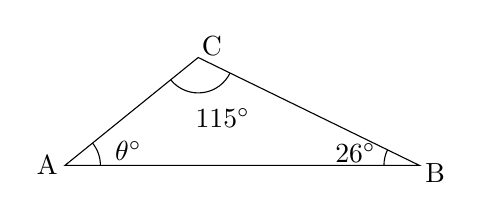
\begin{tikzpicture}[scale=1.5, baseline=(current bounding box.north)]
      \pgfmathsetmacro{\angleA}{39}
      \pgfmathsetmacro{\angleB}{26}
      \pgfmathsetmacro{\angleC}{115}
      \pgfmathsetmacro{\sideC}{3}
      \pgfmathsetmacro{\rotationAngle}{0}


      \begin{scope}[rotate=\rotationAngle]
        \coordinate (A) at (0,0);
        \coordinate (B) at (\sideC,0);
        \coordinate (C) at (intersection cs: first line={(A)--($(A)+(\angleA:4cm)$)}, second line={(B)--($(B)+(180-\angleB:4cm)$)});
        \draw (A) -- (B) -- (C) -- cycle;

        % Mark angles with arcs
        \draw ($(A)!0.3cm!(B)$) arc [start angle=0, end angle=\angleA, radius=0.3cm];
        \draw ($(B)!0.3cm!(C)$) arc [start angle=180-\angleB, end angle=180, radius=0.3cm];
        \draw ($(C)!0.3cm!(A)$) arc [start angle=180+\angleA, end angle=360-\angleB, radius=0.3cm];

        % Label angles
        \node at ($(A)!-0.15cm!(B)$) {A};
        \node at ($(B)!-0.15cm!(C)$) {B};
        \node at ($(C)!-0.15cm!(A)$) {C};

        % Mark angles in degrees
        \coordinate (midBC) at ($(B)!0.5!(C)$);
        \node at ($(A)!0.55cm!(midBC)$) {$\theta ^\circ$};

        \coordinate (midAC) at ($(A)!0.5!(C)$);
        \node at ($(B)!0.55cm!(midAC)$) {26$^\circ$};

        \coordinate (midAB) at ($(A)!0.5!(B)$);
        \node at ($(C)!0.55cm!(midAB)$) {115$^\circ$};

      \end{scope}
    \end{tikzpicture}
\end{minipage}%
\hfill
\begin{minipage}{0.4\textwidth}
    \begin{align*}
        \angle \text{A} &= 180^\circ - (\angle \text{B} + \angle \text{C}) \\
        &= 180^\circ - (\dotuline{~~~~~~~}^\circ + \dotuline{~~~~~~~}^\circ) \\
        &= 180^\circ - \dotuline{~~~~~~~}^\circ \\
        &= \dotuline{~~~~~~~}^\circ
    \end{align*}
\end{minipage}

\vspace{1cm}\begin{minipage}{0.55\textwidth}
  \refstepcounter{minipagecount}
  \noindent{(\theminipagecount)}\quad
  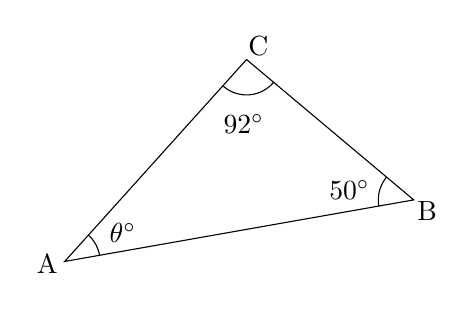
\begin{tikzpicture}[scale=1.5, baseline=(current bounding box.north)]
      \pgfmathsetmacro{\angleA}{38}
      \pgfmathsetmacro{\angleB}{50}
      \pgfmathsetmacro{\angleC}{92}
      \pgfmathsetmacro{\sideC}{3}
      \pgfmathsetmacro{\rotationAngle}{10}


      \begin{scope}[rotate=\rotationAngle]
        \coordinate (A) at (0,0);
        \coordinate (B) at (\sideC,0);
        \coordinate (C) at (intersection cs: first line={(A)--($(A)+(\angleA:4cm)$)}, second line={(B)--($(B)+(180-\angleB:4cm)$)});
        \draw (A) -- (B) -- (C) -- cycle;

        % Mark angles with arcs
        \draw ($(A)!0.3cm!(B)$) arc [start angle=0, end angle=\angleA, radius=0.3cm];
        \draw ($(B)!0.3cm!(C)$) arc [start angle=180-\angleB, end angle=180, radius=0.3cm];
        \draw ($(C)!0.3cm!(A)$) arc [start angle=180+\angleA, end angle=360-\angleB, radius=0.3cm];

        % Label angles
        \node at ($(A)!-0.15cm!(B)$) {A};
        \node at ($(B)!-0.15cm!(C)$) {B};
        \node at ($(C)!-0.15cm!(A)$) {C};

        % Mark angles in degrees
        \coordinate (midBC) at ($(B)!0.5!(C)$);
        \node at ($(A)!0.55cm!(midBC)$) {$\theta ^\circ$};

        \coordinate (midAC) at ($(A)!0.5!(C)$);
        \node at ($(B)!0.55cm!(midAC)$) {50$^\circ$};

        \coordinate (midAB) at ($(A)!0.5!(B)$);
        \node at ($(C)!0.55cm!(midAB)$) {92$^\circ$};

      \end{scope}
    \end{tikzpicture}
\end{minipage}%
\hfill
\begin{minipage}{0.4\textwidth}
    \begin{align*}
        \angle \text{A} &= 180^\circ - (\angle \text{B} + \angle \text{C}) \\
        &= 180^\circ - (\dotuline{~~~~~~~}^\circ + \dotuline{~~~~~~~}^\circ) \\
        &= 180^\circ - \dotuline{~~~~~~~}^\circ \\
        &= \dotuline{~~~~~~~}^\circ
    \end{align*}
\end{minipage}

\vspace{1cm}\begin{minipage}{0.55\textwidth}
  \refstepcounter{minipagecount}
  \noindent{(\theminipagecount)}\quad
  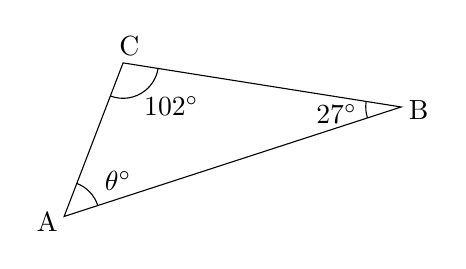
\begin{tikzpicture}[scale=1.5, baseline=(current bounding box.north)]
      \pgfmathsetmacro{\angleA}{51}
      \pgfmathsetmacro{\angleB}{27}
      \pgfmathsetmacro{\angleC}{102}
      \pgfmathsetmacro{\sideC}{3}
      \pgfmathsetmacro{\rotationAngle}{18}


      \begin{scope}[rotate=\rotationAngle]
        \coordinate (A) at (0,0);
        \coordinate (B) at (\sideC,0);
        \coordinate (C) at (intersection cs: first line={(A)--($(A)+(\angleA:4cm)$)}, second line={(B)--($(B)+(180-\angleB:4cm)$)});
        \draw (A) -- (B) -- (C) -- cycle;

        % Mark angles with arcs
        \draw ($(A)!0.3cm!(B)$) arc [start angle=0, end angle=\angleA, radius=0.3cm];
        \draw ($(B)!0.3cm!(C)$) arc [start angle=180-\angleB, end angle=180, radius=0.3cm];
        \draw ($(C)!0.3cm!(A)$) arc [start angle=180+\angleA, end angle=360-\angleB, radius=0.3cm];

        % Label angles
        \node at ($(A)!-0.15cm!(B)$) {A};
        \node at ($(B)!-0.15cm!(C)$) {B};
        \node at ($(C)!-0.15cm!(A)$) {C};

        % Mark angles in degrees
        \coordinate (midBC) at ($(B)!0.5!(C)$);
        \node at ($(A)!0.55cm!(midBC)$) {$\theta ^\circ$};

        \coordinate (midAC) at ($(A)!0.5!(C)$);
        \node at ($(B)!0.55cm!(midAC)$) {27$^\circ$};

        \coordinate (midAB) at ($(A)!0.5!(B)$);
        \node at ($(C)!0.55cm!(midAB)$) {102$^\circ$};

      \end{scope}
    \end{tikzpicture}
\end{minipage}%
\hfill
\begin{minipage}{0.4\textwidth}
    \begin{align*}
        \angle \text{A} &= 180^\circ - (\angle \text{B} + \angle \text{C}) \\
        &= 180^\circ - (\dotuline{~~~~~~~}^\circ + \dotuline{~~~~~~~}^\circ) \\
        &= 180^\circ - \dotuline{~~~~~~~}^\circ \\
        &= \dotuline{~~~~~~~}^\circ
    \end{align*}
\end{minipage}

\vspace{1cm}\begin{minipage}{0.55\textwidth}
  \refstepcounter{minipagecount}
  \noindent{(\theminipagecount)}\quad
  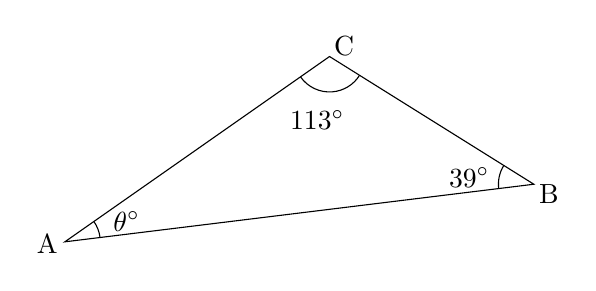
\begin{tikzpicture}[scale=1.5, baseline=(current bounding box.north)]
      \pgfmathsetmacro{\angleA}{28}
      \pgfmathsetmacro{\angleB}{39}
      \pgfmathsetmacro{\angleC}{113}
      \pgfmathsetmacro{\sideC}{4}
      \pgfmathsetmacro{\rotationAngle}{7}


      \begin{scope}[rotate=\rotationAngle]
        \coordinate (A) at (0,0);
        \coordinate (B) at (\sideC,0);
        \coordinate (C) at (intersection cs: first line={(A)--($(A)+(\angleA:4cm)$)}, second line={(B)--($(B)+(180-\angleB:4cm)$)});
        \draw (A) -- (B) -- (C) -- cycle;

        % Mark angles with arcs
        \draw ($(A)!0.3cm!(B)$) arc [start angle=0, end angle=\angleA, radius=0.3cm];
        \draw ($(B)!0.3cm!(C)$) arc [start angle=180-\angleB, end angle=180, radius=0.3cm];
        \draw ($(C)!0.3cm!(A)$) arc [start angle=180+\angleA, end angle=360-\angleB, radius=0.3cm];

        % Label angles
        \node at ($(A)!-0.15cm!(B)$) {A};
        \node at ($(B)!-0.15cm!(C)$) {B};
        \node at ($(C)!-0.15cm!(A)$) {C};

        % Mark angles in degrees
        \coordinate (midBC) at ($(B)!0.5!(C)$);
        \node at ($(A)!0.55cm!(midBC)$) {$\theta ^\circ$};

        \coordinate (midAC) at ($(A)!0.5!(C)$);
        \node at ($(B)!0.55cm!(midAC)$) {39$^\circ$};

        \coordinate (midAB) at ($(A)!0.5!(B)$);
        \node at ($(C)!0.55cm!(midAB)$) {113$^\circ$};

      \end{scope}
    \end{tikzpicture}
\end{minipage}%
\hfill
\begin{minipage}{0.4\textwidth}
    \begin{align*}
        \angle \text{A} &= 180^\circ - (\angle \text{B} + \angle \text{C}) \\
        &= 180^\circ - (\dotuline{~~~~~~~}^\circ + \dotuline{~~~~~~~}^\circ) \\
        &= 180^\circ - \dotuline{~~~~~~~}^\circ \\
        &= \dotuline{~~~~~~~}^\circ
    \end{align*}
\end{minipage}

\vspace{1cm}\begin{minipage}{0.55\textwidth}
  \refstepcounter{minipagecount}
  \noindent{(\theminipagecount)}\quad
  \begin{tikzpicture}[scale=1.5, baseline=(current bounding box.north)]
      \pgfmathsetmacro{\angleA}{54}
      \pgfmathsetmacro{\angleB}{43}
      \pgfmathsetmacro{\angleC}{83}
      \pgfmathsetmacro{\sideC}{4}
      \pgfmathsetmacro{\rotationAngle}{18}


      \begin{scope}[rotate=\rotationAngle]
        \coordinate (A) at (0,0);
        \coordinate (B) at (\sideC,0);
        \coordinate (C) at (intersection cs: first line={(A)--($(A)+(\angleA:4cm)$)}, second line={(B)--($(B)+(180-\angleB:4cm)$)});
        \draw (A) -- (B) -- (C) -- cycle;

        % Mark angles with arcs
        \draw ($(A)!0.3cm!(B)$) arc [start angle=0, end angle=\angleA, radius=0.3cm];
        \draw ($(B)!0.3cm!(C)$) arc [start angle=180-\angleB, end angle=180, radius=0.3cm];
        \draw ($(C)!0.3cm!(A)$) arc [start angle=180+\angleA, end angle=360-\angleB, radius=0.3cm];

        % Label angles
        \node at ($(A)!-0.15cm!(B)$) {A};
        \node at ($(B)!-0.15cm!(C)$) {B};
        \node at ($(C)!-0.15cm!(A)$) {C};

        % Mark angles in degrees
        \coordinate (midBC) at ($(B)!0.5!(C)$);
        \node at ($(A)!0.55cm!(midBC)$) {$\theta ^\circ$};

        \coordinate (midAC) at ($(A)!0.5!(C)$);
        \node at ($(B)!0.55cm!(midAC)$) {43$^\circ$};

        \coordinate (midAB) at ($(A)!0.5!(B)$);
        \node at ($(C)!0.55cm!(midAB)$) {83$^\circ$};

      \end{scope}
    \end{tikzpicture}
\end{minipage}%
\hfill
\begin{minipage}{0.4\textwidth}
    \begin{align*}
        \angle \text{A} &= 180^\circ - (\angle \text{B} + \angle \text{C}) \\
        &= 180^\circ - (\dotuline{~~~~~~~}^\circ + \dotuline{~~~~~~~}^\circ) \\
        &= 180^\circ - \dotuline{~~~~~~~}^\circ \\
        &= \dotuline{~~~~~~~}^\circ
    \end{align*}
\end{minipage}

\vspace{1cm}\begin{minipage}{0.55\textwidth}
  \refstepcounter{minipagecount}
  \noindent{(\theminipagecount)}\quad
  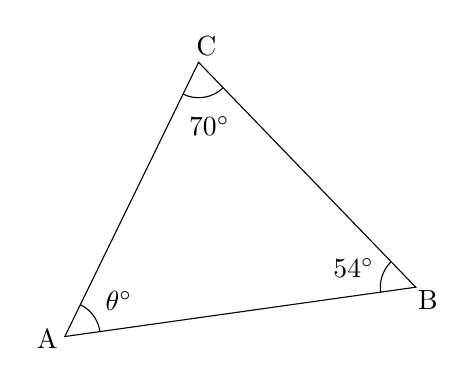
\begin{tikzpicture}[scale=1.5, baseline=(current bounding box.north)]
      \pgfmathsetmacro{\angleA}{56}
      \pgfmathsetmacro{\angleB}{54}
      \pgfmathsetmacro{\angleC}{70}
      \pgfmathsetmacro{\sideC}{3}
      \pgfmathsetmacro{\rotationAngle}{8}


      \begin{scope}[rotate=\rotationAngle]
        \coordinate (A) at (0,0);
        \coordinate (B) at (\sideC,0);
        \coordinate (C) at (intersection cs: first line={(A)--($(A)+(\angleA:4cm)$)}, second line={(B)--($(B)+(180-\angleB:4cm)$)});
        \draw (A) -- (B) -- (C) -- cycle;

        % Mark angles with arcs
        \draw ($(A)!0.3cm!(B)$) arc [start angle=0, end angle=\angleA, radius=0.3cm];
        \draw ($(B)!0.3cm!(C)$) arc [start angle=180-\angleB, end angle=180, radius=0.3cm];
        \draw ($(C)!0.3cm!(A)$) arc [start angle=180+\angleA, end angle=360-\angleB, radius=0.3cm];

        % Label angles
        \node at ($(A)!-0.15cm!(B)$) {A};
        \node at ($(B)!-0.15cm!(C)$) {B};
        \node at ($(C)!-0.15cm!(A)$) {C};

        % Mark angles in degrees
        \coordinate (midBC) at ($(B)!0.5!(C)$);
        \node at ($(A)!0.55cm!(midBC)$) {$\theta ^\circ$};

        \coordinate (midAC) at ($(A)!0.5!(C)$);
        \node at ($(B)!0.55cm!(midAC)$) {54$^\circ$};

        \coordinate (midAB) at ($(A)!0.5!(B)$);
        \node at ($(C)!0.55cm!(midAB)$) {70$^\circ$};

      \end{scope}
    \end{tikzpicture}
\end{minipage}%
\hfill
\begin{minipage}{0.4\textwidth}
    \begin{align*}
        \angle \text{A} &= 180^\circ - (\angle \text{B} + \angle \text{C}) \\
        &= 180^\circ - (\dotuline{~~~~~~~}^\circ + \dotuline{~~~~~~~}^\circ) \\
        &= 180^\circ - \dotuline{~~~~~~~}^\circ \\
        &= \dotuline{~~~~~~~}^\circ
    \end{align*}
\end{minipage}

\vspace{1cm}\begin{minipage}{0.55\textwidth}
  \refstepcounter{minipagecount}
  \noindent{(\theminipagecount)}\quad
  \begin{tikzpicture}[scale=1.5, baseline=(current bounding box.north)]
      \pgfmathsetmacro{\angleA}{48}
      \pgfmathsetmacro{\angleB}{60}
      \pgfmathsetmacro{\angleC}{72}
      \pgfmathsetmacro{\sideC}{4}
      \pgfmathsetmacro{\rotationAngle}{7}


      \begin{scope}[rotate=\rotationAngle]
        \coordinate (A) at (0,0);
        \coordinate (B) at (\sideC,0);
        \coordinate (C) at (intersection cs: first line={(A)--($(A)+(\angleA:4cm)$)}, second line={(B)--($(B)+(180-\angleB:4cm)$)});
        \draw (A) -- (B) -- (C) -- cycle;

        % Mark angles with arcs
        \draw ($(A)!0.3cm!(B)$) arc [start angle=0, end angle=\angleA, radius=0.3cm];
        \draw ($(B)!0.3cm!(C)$) arc [start angle=180-\angleB, end angle=180, radius=0.3cm];
        \draw ($(C)!0.3cm!(A)$) arc [start angle=180+\angleA, end angle=360-\angleB, radius=0.3cm];

        % Label angles
        \node at ($(A)!-0.15cm!(B)$) {A};
        \node at ($(B)!-0.15cm!(C)$) {B};
        \node at ($(C)!-0.15cm!(A)$) {C};

        % Mark angles in degrees
        \coordinate (midBC) at ($(B)!0.5!(C)$);
        \node at ($(A)!0.55cm!(midBC)$) {$\theta ^\circ$};

        \coordinate (midAC) at ($(A)!0.5!(C)$);
        \node at ($(B)!0.55cm!(midAC)$) {60$^\circ$};

        \coordinate (midAB) at ($(A)!0.5!(B)$);
        \node at ($(C)!0.55cm!(midAB)$) {72$^\circ$};

      \end{scope}
    \end{tikzpicture}
\end{minipage}%
\hfill
\begin{minipage}{0.4\textwidth}
    \begin{align*}
        \angle \text{A} &= 180^\circ - (\angle \text{B} + \angle \text{C}) \\
        &= 180^\circ - (\dotuline{~~~~~~~}^\circ + \dotuline{~~~~~~~}^\circ) \\
        &= 180^\circ - \dotuline{~~~~~~~}^\circ \\
        &= \dotuline{~~~~~~~}^\circ
    \end{align*}
\end{minipage}

\vspace{1cm}\begin{minipage}{0.55\textwidth}
  \refstepcounter{minipagecount}
  \noindent{(\theminipagecount)}\quad
  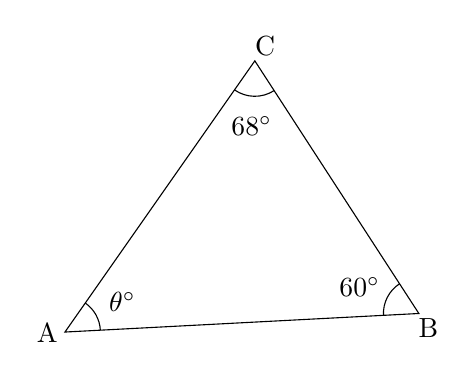
\begin{tikzpicture}[scale=1.5, baseline=(current bounding box.north)]
      \pgfmathsetmacro{\angleA}{52}
      \pgfmathsetmacro{\angleB}{60}
      \pgfmathsetmacro{\angleC}{68}
      \pgfmathsetmacro{\sideC}{3}
      \pgfmathsetmacro{\rotationAngle}{3}


      \begin{scope}[rotate=\rotationAngle]
        \coordinate (A) at (0,0);
        \coordinate (B) at (\sideC,0);
        \coordinate (C) at (intersection cs: first line={(A)--($(A)+(\angleA:4cm)$)}, second line={(B)--($(B)+(180-\angleB:4cm)$)});
        \draw (A) -- (B) -- (C) -- cycle;

        % Mark angles with arcs
        \draw ($(A)!0.3cm!(B)$) arc [start angle=0, end angle=\angleA, radius=0.3cm];
        \draw ($(B)!0.3cm!(C)$) arc [start angle=180-\angleB, end angle=180, radius=0.3cm];
        \draw ($(C)!0.3cm!(A)$) arc [start angle=180+\angleA, end angle=360-\angleB, radius=0.3cm];

        % Label angles
        \node at ($(A)!-0.15cm!(B)$) {A};
        \node at ($(B)!-0.15cm!(C)$) {B};
        \node at ($(C)!-0.15cm!(A)$) {C};

        % Mark angles in degrees
        \coordinate (midBC) at ($(B)!0.5!(C)$);
        \node at ($(A)!0.55cm!(midBC)$) {$\theta ^\circ$};

        \coordinate (midAC) at ($(A)!0.5!(C)$);
        \node at ($(B)!0.55cm!(midAC)$) {60$^\circ$};

        \coordinate (midAB) at ($(A)!0.5!(B)$);
        \node at ($(C)!0.55cm!(midAB)$) {68$^\circ$};

      \end{scope}
    \end{tikzpicture}
\end{minipage}%
\hfill
\begin{minipage}{0.4\textwidth}
    \begin{align*}
        \angle \text{A} &= 180^\circ - (\angle \text{B} + \angle \text{C}) \\
        &= 180^\circ - (\dotuline{~~~~~~~}^\circ + \dotuline{~~~~~~~}^\circ) \\
        &= 180^\circ - \dotuline{~~~~~~~}^\circ \\
        &= \dotuline{~~~~~~~}^\circ
    \end{align*}
\end{minipage}

\vspace{1cm}\begin{minipage}{0.55\textwidth}
  \refstepcounter{minipagecount}
  \noindent{(\theminipagecount)}\quad
  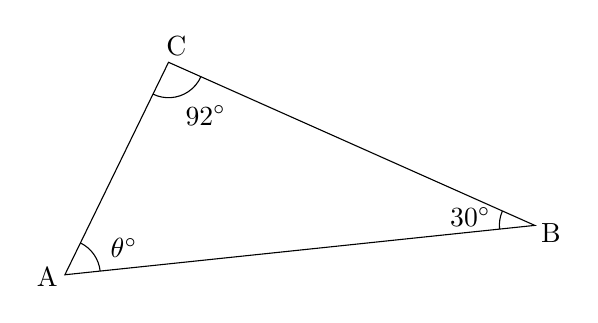
\begin{tikzpicture}[scale=1.5, baseline=(current bounding box.north)]
      \pgfmathsetmacro{\angleA}{58}
      \pgfmathsetmacro{\angleB}{30}
      \pgfmathsetmacro{\angleC}{92}
      \pgfmathsetmacro{\sideC}{4}
      \pgfmathsetmacro{\rotationAngle}{6}


      \begin{scope}[rotate=\rotationAngle]
        \coordinate (A) at (0,0);
        \coordinate (B) at (\sideC,0);
        \coordinate (C) at (intersection cs: first line={(A)--($(A)+(\angleA:4cm)$)}, second line={(B)--($(B)+(180-\angleB:4cm)$)});
        \draw (A) -- (B) -- (C) -- cycle;

        % Mark angles with arcs
        \draw ($(A)!0.3cm!(B)$) arc [start angle=0, end angle=\angleA, radius=0.3cm];
        \draw ($(B)!0.3cm!(C)$) arc [start angle=180-\angleB, end angle=180, radius=0.3cm];
        \draw ($(C)!0.3cm!(A)$) arc [start angle=180+\angleA, end angle=360-\angleB, radius=0.3cm];

        % Label angles
        \node at ($(A)!-0.15cm!(B)$) {A};
        \node at ($(B)!-0.15cm!(C)$) {B};
        \node at ($(C)!-0.15cm!(A)$) {C};

        % Mark angles in degrees
        \coordinate (midBC) at ($(B)!0.5!(C)$);
        \node at ($(A)!0.55cm!(midBC)$) {$\theta ^\circ$};

        \coordinate (midAC) at ($(A)!0.5!(C)$);
        \node at ($(B)!0.55cm!(midAC)$) {30$^\circ$};

        \coordinate (midAB) at ($(A)!0.5!(B)$);
        \node at ($(C)!0.55cm!(midAB)$) {92$^\circ$};

      \end{scope}
    \end{tikzpicture}
\end{minipage}%
\hfill
\begin{minipage}{0.4\textwidth}
    \begin{align*}
        \angle \text{A} &= 180^\circ - (\angle \text{B} + \angle \text{C}) \\
        &= 180^\circ - (\dotuline{~~~~~~~}^\circ + \dotuline{~~~~~~~}^\circ) \\
        &= 180^\circ - \dotuline{~~~~~~~}^\circ \\
        &= \dotuline{~~~~~~~}^\circ
    \end{align*}
\end{minipage}

\vspace{1cm}\begin{minipage}{0.55\textwidth}
  \refstepcounter{minipagecount}
  \noindent{(\theminipagecount)}\quad
  \begin{tikzpicture}[scale=1.5, baseline=(current bounding box.north)]
      \pgfmathsetmacro{\angleA}{38}
      \pgfmathsetmacro{\angleB}{57}
      \pgfmathsetmacro{\angleC}{85}
      \pgfmathsetmacro{\sideC}{4}
      \pgfmathsetmacro{\rotationAngle}{14}


      \begin{scope}[rotate=\rotationAngle]
        \coordinate (A) at (0,0);
        \coordinate (B) at (\sideC,0);
        \coordinate (C) at (intersection cs: first line={(A)--($(A)+(\angleA:4cm)$)}, second line={(B)--($(B)+(180-\angleB:4cm)$)});
        \draw (A) -- (B) -- (C) -- cycle;

        % Mark angles with arcs
        \draw ($(A)!0.3cm!(B)$) arc [start angle=0, end angle=\angleA, radius=0.3cm];
        \draw ($(B)!0.3cm!(C)$) arc [start angle=180-\angleB, end angle=180, radius=0.3cm];
        \draw ($(C)!0.3cm!(A)$) arc [start angle=180+\angleA, end angle=360-\angleB, radius=0.3cm];

        % Label angles
        \node at ($(A)!-0.15cm!(B)$) {A};
        \node at ($(B)!-0.15cm!(C)$) {B};
        \node at ($(C)!-0.15cm!(A)$) {C};

        % Mark angles in degrees
        \coordinate (midBC) at ($(B)!0.5!(C)$);
        \node at ($(A)!0.55cm!(midBC)$) {$\theta ^\circ$};

        \coordinate (midAC) at ($(A)!0.5!(C)$);
        \node at ($(B)!0.55cm!(midAC)$) {57$^\circ$};

        \coordinate (midAB) at ($(A)!0.5!(B)$);
        \node at ($(C)!0.55cm!(midAB)$) {85$^\circ$};

      \end{scope}
    \end{tikzpicture}
\end{minipage}%
\hfill
\begin{minipage}{0.4\textwidth}
    \begin{align*}
        \angle \text{A} &= 180^\circ - (\angle \text{B} + \angle \text{C}) \\
        &= 180^\circ - (\dotuline{~~~~~~~}^\circ + \dotuline{~~~~~~~}^\circ) \\
        &= 180^\circ - \dotuline{~~~~~~~}^\circ \\
        &= \dotuline{~~~~~~~}^\circ
    \end{align*}
\end{minipage}

\vspace{1cm}\begin{minipage}{0.55\textwidth}
  \refstepcounter{minipagecount}
  \noindent{(\theminipagecount)}\quad
  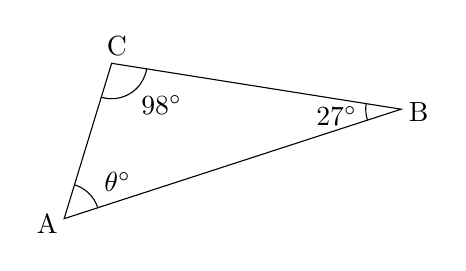
\begin{tikzpicture}[scale=1.5, baseline=(current bounding box.north)]
      \pgfmathsetmacro{\angleA}{55}
      \pgfmathsetmacro{\angleB}{27}
      \pgfmathsetmacro{\angleC}{98}
      \pgfmathsetmacro{\sideC}{3}
      \pgfmathsetmacro{\rotationAngle}{18}


      \begin{scope}[rotate=\rotationAngle]
        \coordinate (A) at (0,0);
        \coordinate (B) at (\sideC,0);
        \coordinate (C) at (intersection cs: first line={(A)--($(A)+(\angleA:4cm)$)}, second line={(B)--($(B)+(180-\angleB:4cm)$)});
        \draw (A) -- (B) -- (C) -- cycle;

        % Mark angles with arcs
        \draw ($(A)!0.3cm!(B)$) arc [start angle=0, end angle=\angleA, radius=0.3cm];
        \draw ($(B)!0.3cm!(C)$) arc [start angle=180-\angleB, end angle=180, radius=0.3cm];
        \draw ($(C)!0.3cm!(A)$) arc [start angle=180+\angleA, end angle=360-\angleB, radius=0.3cm];

        % Label angles
        \node at ($(A)!-0.15cm!(B)$) {A};
        \node at ($(B)!-0.15cm!(C)$) {B};
        \node at ($(C)!-0.15cm!(A)$) {C};

        % Mark angles in degrees
        \coordinate (midBC) at ($(B)!0.5!(C)$);
        \node at ($(A)!0.55cm!(midBC)$) {$\theta ^\circ$};

        \coordinate (midAC) at ($(A)!0.5!(C)$);
        \node at ($(B)!0.55cm!(midAC)$) {27$^\circ$};

        \coordinate (midAB) at ($(A)!0.5!(B)$);
        \node at ($(C)!0.55cm!(midAB)$) {98$^\circ$};

      \end{scope}
    \end{tikzpicture}
\end{minipage}%
\hfill
\begin{minipage}{0.4\textwidth}
    \begin{align*}
        \angle \text{A} &= 180^\circ - (\angle \text{B} + \angle \text{C}) \\
        &= 180^\circ - (\dotuline{~~~~~~~}^\circ + \dotuline{~~~~~~~}^\circ) \\
        &= 180^\circ - \dotuline{~~~~~~~}^\circ \\
        &= \dotuline{~~~~~~~}^\circ
    \end{align*}
\end{minipage}

\vspace{1cm}

\end{document}
